%
% main.tex -- Paper zum Thema <maxwell>
%
% (c) 2020 Autor, OST Ostschweizer Fachhochschule
%
% !TEX root = ../../buch.tex
% !TEX encoding = UTF-8
%

\chapter{Maxwell-Gleichungen als Variationsprinzip\label{chapter:maxwell}}
\kopflinks{Maxwell-Gleichungen als Variationsprinzip}
\begin{refsection}
\chapterauthor{Maurin Doswald und Stephan Oseghale}

Als James Clerk Maxwell 1865 seine Arbeit über das elektromagnetische Feld veröffentlichte, gelang es ihm, das Wesen des elektrischen- und magnetischen Feldes, sowie die Interaktion derselben mathematisch zu beschreiben und somit das Grundwesen der Elektrodynamik aufzuzeigen.
Durch seine theoretische Arbeit konnte experimentell die Existenz von elektromagnetischen Wellen und ihre Ausbreitung mit Lichtgeschwindigkeit nachgewiesen werden.
Dies führte zu Technologien wie Radio, Radar, Fernsehen, Antennen (Kapitel \ref{chapter:antennen}) und viele weitere Anwendungen in der drahtlosen Kommunikation. 
%Eine detaillierte Untersuchung einer weiteren Anwendung wird im Kapitel \ref{chapter:antennen} über Antennen behandelt.

Die Grundidee zur Formulierung dieser Gleichungen kam durch eine Reihe von experimentellen Beobachtungen und theoretischen Ansätzen unterschiedlichster Wissenschaftler unter anderem Michael Faraday und André-Marie Ampère.
Durch mathematische Analysen und Experimente entwickelte Maxwell schlussendlich 20 Gleichungen, welche später von Oliver Heavyside und Willard Gibbs in die heutige bekannte vektorielle Schreibweise von vier Gleichungen gebracht wurden.
Das Ziel dieser Arbeit ist aufzuzeigen, dass die vier fundamentalen Gleichungen  auch über ein Variationsprinzip hergeleitet werden können.

%
% mathFormulierung.tex -- Felder und deren Operationen
%
% 
%
% !TEX root = ../../buch.tex
% !TEX encoding = UTF-8
%
\section{Felder\label{maxwell:mathFormulierung}}
\rhead{Felder}

Da sowohl das elektrische Feld $\vec{E}$ wie auch das magnetische Feld bzw. die magnetische Flussdichte $\vec{B}$ als Vektorfeld beschrieben werden, soll hier der Begriff des Feldes erläutert und grafisch aufgezeigt werden.

\subsection{Skalarfeld\label{maxwell:skalarfeld}}

Ein Skalarfeld ist eine Funktion der Form
\( f:\mathbb{R}^n \rightarrow \mathbb{R}, \) 
die jedem Punkt im Raum ein Skalar zuordnet.
Alltägliche Beispiele für Skalarfelder sind Temperaturverteilungen, Ladungsdichten oder Potentiale. In Abbildung \ref{maxwell:skalarGrad} ist ein Skalarfeld abgebildet.


%Zu den wichtigsten Operationen eines Skalarfeldes gehört der Gradient, welcher dem Skalar- ein Vektorfeld zuordnet.
%Sei $\phi$ ein Skalarfeld, dann ist $\nabla\phi$ ein Vektorfeld, dargestellt in \ref{maxwell:skalarGrad}.

\begin{figure}
	\centering
	\begin{subfigure}{0.50\textwidth}
	%\subfigure{\includegraphics[width=0.50\textwidth]{papers/maxwell/skalar}}
	\includegraphics[width=\textwidth]{papers/maxwell/skalar}
	\end{subfigure}
	%\subfigure{\includegraphics[width=0.45\textwidth]{papers/maxwell/gradient}}
	\begin{subfigure}{0.45\textwidth}
	\includegraphics[width=\textwidth]{papers/maxwell/gradient}
	\end{subfigure}
	\caption{Skalar- und Vektorfeld}
	\label{maxwell:skalarGrad}
\end{figure}

\subsection{Vektorfeld\label{maxwell:vektorfeld}}

Ein Vektorfeld ist eine Funktion der Form \( f: \mathbb{R}^n \rightarrow \mathbb{R}^m, \) welche jedem Punkt im Raum einen Vektor zuweist. 
Die Richtung dieses Vektors gibt hierbei an, in welche Richtung der Fluss des Feldes an diesem Punkt geht, während der Betrag die Intensität repräsentiert.


Des weiteren spricht man von einem stationären Vektorfeld, wenn es zeitunabhängig ist und von einem homogenen Vektorfeld, wenn die Richtung und der Betrag der Vektoren ortsunabhängig sind, also wenn jeder Vektor die gleiche Richtung und den gleichen Betrag hat. 
Wie bereits erwähnt, sind das elektrische und das magnetische Feld, wie auch andere Kraftfelder Beispiele von Vektorfeldern.
In Abbildung \ref{maxwell:skalarGrad} ist ein Vektorfeld abgebildet.

\subsection{Operationen}

\subsubsection{Gradient}

Der Gradient einer Funktion $f:\mathbb{R}^3 \rightarrow \mathbb{R}$ ist als 
\[
\renewcommand{\arraystretch}{1.9} 
\operatorname{grad}f = \nabla f = \begin{pmatrix}
\displaystyle
\frac{\partial f}{\partial x} \\
\displaystyle
\frac{\partial f}{\partial y} \\
\displaystyle
\frac{\partial f}{\partial z} \\
\end{pmatrix}\] 
definiert und wurde bereits in Abschnitt \ref{buch:fuvar:richtungsableitung:def:gradient} genauer behandelt. Dieser Operator wird auf ein Skalarfeld angewendet und resultiert in einem Vektorfeld. 
Die Richtung der Vektoren dieses neuen Vektorfeldes zeigen immer in die Richtung der grössten bzw. steilsten Zunahme, wobei der Betrag die Steilheit des Anstiegs repräsentiert.
%Weiter unten wird ersichtlich, dass auch das elektrische Feld ein Gradientenfeld ist \[ \vec{E} = -\nabla\varphi, \] wobei $\varphi$ das elektrische Potential ist.

\subsubsection{Divergenz}
%TODO: Link auf Kapitel von Müller
Die Divergenz eines Vektorfeldes $\vec{F}:\mathbb{R}^3 \rightarrow \mathbb{R}^3$ ist definiert als 
\[ \operatorname{div}\vec{F} = \nabla\cdot\vec{F} 
= \frac{\partial F_x}{\partial x} + \frac{\partial F_y}{\partial y} + \frac{\partial F_z}{\partial z}. \]
Angewendet wird sie auf ein Vektorfeld und es resultiert ein Skalarfeld.
Die Divergenz sagt aus, ob an einem Punkt mehr ``hinein-'' als ``herausfliesst'' und macht so eine Aussage über das Bestehen von Quellen und Senken. 
Wenn die Divergenz negativ ist, liegt eine Senke vor, wenn sie positiv ist eine Quelle.
Ein Vektorfeld wird als quellenfrei bezeichnet, wenn seine Divergenz gleich null ist.

\subsubsection{Rotation}
%TODO: Link auf Kapitel von Müller
Die Rotation eines Vektorfeldes $\vec{F}:\mathbb{R}^3 \rightarrow \mathbb{R}^3$ ist definiert als
\[
\renewcommand{\arraystretch}{1.9} 
\operatorname{rot}\vec{F} = 
\operatorname{curl}\vec{F}
=\nabla\times\vec{F}
= \begin{pmatrix}
	\displaystyle
	\frac{\partial F_z}{\partial y} -\frac{\partial F_y}{\partial z}\\
	\displaystyle
	\frac{\partial F_x}{\partial z} -\frac{\partial F_z}{\partial x}\\
	\displaystyle
	\frac{\partial F_y}{\partial x} -\frac{\partial F_x}{\partial y}
\end{pmatrix}
. \]
Mit dieser Operation wird einem Vektorfeld ein neues Vektorfeld zugeordnet, welches eine Aussage darüber macht, wie stark das Feld sich um einen Punkt dreht bzw. rotiert.
Ein Vektorfeld ist wirbelfrei, wenn seine Rotation null ist.

%
% einleitung.tex -- Beispiel-File für die Einleitung
%
% (c) 2020 Prof Dr Andreas Müller, Hochschule Rapperswil
%
% !TEX root = ../../buch.tex
% !TEX encoding = UTF-8
%
% erste Maxwellgleichung ohne Quelle

\section{Elektrostatik\label{maxwell:section:elekktrostatik}}
\rhead{Elektrostatik}
Die Elektrostatik ist ein Spezialfall der Elektrodynamik, bei dem statische, das heisst zeitlich nicht veränderliche Felder betrachtet werden.
Dies setzt voraus, dass
\begin{equation}
	\frac{\partial f}{\partial t}
	=
	0
	\label{maxwell:section:definition_statik}
\end{equation}
für alle Funktionen gilt, welche wir in diesem Abschnitt betrachten.
Daraus folgt, dass uns nur ruhende Ladungen interessieren.
Dies hat zur Folge, dass keine Stromdichten existieren können, weil
\begin{equation}
	\varrho\,\vec{v}
	=
	\varrho\, \underbrace{\frac{\partial \vec{x}}{\partial t}}_{=0}
	=
	\vec{\jmath}
	=
	0.
\end{equation}
Im späteren Abschnitt \ref{maxwell:magnetostatik} der Magnetostatik wird klar, dass aus diesem Grund in der Elektrostatik keine magnetische Flussdichte existieren kann.
 
Das Ziel ist nun, das elektrische Feld im Zusammenspiel mit ruhenden Ladungen zu beschreiben.
Dafür werden wir in den folgenden Abschnitten die nötigen Begriffe definieren und genauer erklären.

\subsubsection{Elektrisches Potentialfeld}
Das elektrische Potentialfeld
\(
\varphi:\mathbb{R}^3
\rightarrow
\mathbb{R}
\)
ist als
\begin{equation}
	\varphi(x,y,z)
	=
	\frac{W_{\text{pot}}(x,y,z)}{q}
	\label{maxwell:section:definition_elektrischespotentialfeld}
\end{equation}
definiert.
In Worten gefasst kann man sagen, dass das elektrische Potential eine auf die Ladung normierte potentielle Energie darstellt.
Somit kann die linke Abbildung in \ref{maxwell:skalarGrad} als ein Feld, das proportional zur potentiellen Energie ist, angeschaut werden.
Des weiteren steht die elektrische Spannung eng in Verbindung mit dem elektrischen Potential.
Die Spannung $U$ zwischen zwei Punkten $a$ und $b$ wird definiert als
\(
U_{ab}
=
\varphi_a - \varphi_b.
\)
% not sure about this
Das heisst die Spannung ist der Potentialunterschied zwischen zwei Punkten.

\subsubsection{Elektrisches Feld}
Das elektrische Feld
\(
\vec{E}:\mathbb{R}^3 \rightarrow \mathbb{R}^3
\)
wird in der Elektrostatik definiert als
\begin{equation}
	\vec{E}
	=
	- \nabla\varphi.
	\label{maxwell:section:definition_statisch_elektrischesFeld}
\end{equation}
Diese Definition besagt, dass das elektrische Feld ein statisches Gradientenfeld ist.
Dieses Feld kann man anhand der Kraftwirkung an sogenannten Probeladungen $q$ messen, da
\[
\vec{E}
=
\frac{\vec{F}}{q}
\]
ist.
Somit sind die Vektoren in Abbildung \ref{maxwell:section:E-Feld_punktladung} Kraftvektoren, welche normiert sind auf die Ladung $q$.
%E-Field of point charge
\begin{figure}
	\centering
	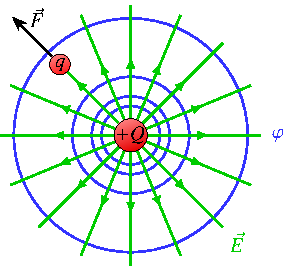
\includegraphics{papers/maxwell/images/pointcharge.pdf}
	\caption{Elektrisches Feld (grün) einer positiven Punktladung $+Q$ und Äquipotentiallinien (blau) der selben positiven Punktladung $+Q$}
	\label{maxwell:section:E-Feld_punktladung}
\end{figure}


\subsubsection{Energiedichte im elektrischen Feld}
Das elektrische Feld beinhaltet eine Energie und somit auch eine Energiedichte.
Diese Energiedichte ist definiert als
\begin{equation}
w_{\text{e}}
=
\frac{1}{2}\,\varepsilon\,\vec{E}\,^2,
\label{maxwell:section:definiton_energiedichte_elektrischesFeld}
\end{equation}
wobei $\varepsilon$ die Permittivität ist.
Die Permittivität
\(
\varepsilon
=
\varepsilon_r\,\varepsilon_0
\)
ist ein Mass dafür, wie gut sich ein Material polarisieren lässt. Es ist das Produkt der relativen Permittivität $\varepsilon_r$ und der Permittivität $\varepsilon_0$ des Vakuums.
Die relative Permittivität ist eine materialabhängige Grösse und hat im Vakuum den skalaren Wert $1$.
Die Permittivität
\[
\varepsilon_0
=
8.854 \cdot 10^{-12}\,\frac{\text{C$^2$}}{\text{Nm$^2$}}
\]
des Vakuums in SI-Einheiten nennt man auch die elektrische Feldkonstante.

\subsection{Laplace-Gleichung
	\label{maxwell:section:elektrostatik_ohne_quelle}}
Man stelle sich nun einen ladungsfreien, luftleeren, drei dimensionalen Raum $V\subset\mathbb{R}^3$
vor, indem ein elektrisches Potentialfeld $\varphi(x,y,z)$ existiert.
Für diesen Raum möchten wir mittels der Variationsrechnung eine partielle Differentialgleichung entwickeln, die beschreibt, wie sich das Potentialfeld und somit auch das elektrische Feld verhält. 

\subsubsection{Ansatz}
Damit wir eine Gleichung erhalten, die das Verhalten des elektrischen Potentialfeldes beschreibt, muss ganz allgemein die Energie im System minimiert werden. 
In diesem Fall ist die Energie im System
\[
W_{\text{e}}
=
\iiint_V w_e\, dV.
\]
Dieses Integral gilt es zu minimieren, was die Grundlage für unser Variationsproblem darstellt.
Die in \eqref{maxwell:section:definiton_energiedichte_elektrischesFeld} definierte Energiedichte ist im Vakuum
\[
w_{\text{e}}
=
\frac{1}{2}\,\varepsilon_0\,\vec{E}\,^2.
\]
Diese Gleichung können wir nun mittels Definition \eqref{maxwell:section:definition_statisch_elektrischesFeld} mit dem elektrischen Potentialfeld ausdrücken.
Folglich ist
\begin{align}
\renewcommand{\arraystretch}{1.9}
w_{\text{e}}
&=
\frac{1}{2}\,\varepsilon_0\left(-\nabla\varphi\right)^2
\\
w_{\text{e}}
&=
\frac{1}{2}\,\varepsilon_0
\begin{pmatrix}
\displaystyle
-\varphi_x\\
\displaystyle
-\varphi_y\\
\displaystyle
-\varphi_z
\end{pmatrix}
\cdot
\begin{pmatrix}
\displaystyle
-\varphi_x\\
\displaystyle
-\varphi_y\\
\displaystyle
-\varphi_z
\end{pmatrix}
=
\frac{1}{2}\,\varepsilon_0\left(\varphi_x^2 + \varphi_y^2 + \varphi_z^2\right).
\label{maxwell:section:energiedichte}
\end{align}
Dies können wir in das zu minimerende Integral einsetzen und bekommen
\begin{equation}
	W_{\text{e}}
	=
	\iiint_V \frac{1}{2}\,\varepsilon_0\left(\varphi_x^2 + \varphi_y^2 + \varphi_z^2\right)\, dV.
	\label{maxwell:section:energieintegral_quellenfrei}
\end{equation}
Aus dieser Gleichung können wir entnehmen, dass unsere Lagrange-Funktion
\begin{equation}
	L(x,y,z,\varphi,\varphi_x,\varphi_y,\varphi_z)
	=
	\frac{1}{2}\,\varepsilon_0\left(\varphi_x^2 + \varphi_y^2 + \varphi_z^2\right)
	\label{maxwell:section:lagrangefunktion_quellenfrei}
\end{equation}
ist.
Somit haben wir unsere Lagrange-Funktion gefunden, die wir in einem nächsten Schritt in die Euler-Ostrogradski-Differentialgleichung einsetzen können.

\subsubsection{Einsetzen in die Euler-Ostrogradski-Differentialgleichung}
Nun gilt es, die in \eqref{maxwell:section:lagrangefunktion_quellenfrei} gefundene Gleichung in die Euler-Ostrogradski-Differentialgleichung \eqref{buch:felder:ostrogradski:eqn:euler-ostrogradski} einzusetzen.
Nach Einsetzen wird die Differentialgleichung zu
\begin{align*}
\frac{1}{2}\,\varepsilon_0\,\biggl(\underbrace{\frac{\partial}{\partial\varphi}\left(\varphi_x^2 + \varphi_y^2 + \varphi_z^2\right)}_{\displaystyle=0} &- \frac{\partial}{\partial x}\frac{\partial}{\partial \varphi_x}\left(\varphi_x^2 + \varphi_y^2 + \varphi_z^2\right)\\
&- \frac{\partial}{\partial y}\frac{\partial}{\partial \varphi_y}\left(\varphi_x^2 + \varphi_y^2 + \varphi_z^2\right) - 
\frac{\partial}{\partial z}\frac{\partial}{\partial \varphi_z}\left(\varphi_x^2 + \varphi_y^2 + \varphi_z^2\right)\biggr)
=
0.
\end{align*}
Man sieht, dass die partielle Ableitung nach $\varphi$ verschwindet.
Nachdem wir die partiellen Ableitungen nach $\varphi_x$, $\varphi_y$ und $\varphi_z$ durchgeführt haben, wird die Differentialgleichung zu
\[
\frac{1}{2}\,\varepsilon_0\left(-\frac{\partial}{\partial x}2\varphi_x - \frac{\partial}{\partial y}2\varphi_y - \frac{\partial}{\partial z}2\varphi_z\right)
=
0.
\]
Wenn man nun noch die letzten partiellen Ableitungen durchführt, resultiert
\begin{equation}
	- \varepsilon_0\underbrace{\left(\frac{\partial^2\varphi}{\partial x^2} + \frac{\partial^2\varphi}{\partial y^2} + \frac{\partial^2\varphi}{\partial z^2}\right)}_{\displaystyle=0}
	=
	0.
	\label{maxwell:section:laplace_gleichung_1}
\end{equation}
%TODO:definiton des laplace operators suchen
An dieser Gleichung sieht man, dass die Klammer mit den partiellen Ableitungen gleich null sein muss, da die Permittivität des Vakuums nicht null sein kann.
Zusätzlich wird nun ersichtlich, dass der Klammerterm nach Definition \eqref{buch:fundamentallemma:definition:laplace-operator} mit dem Laplace-Operator angewendet auf das elektrische Potentialfeld $\varphi$ ersetzt werden kann.
Somit wird unsere Schlussdifferentialgleichung zu
\begin{equation}
	\Delta\varphi
	=
	0.
	\label{maxwell:section:laplace_gleichung_2}
\end{equation}
%TODO: Definition Laplace suchen.
Wenn wir nun den Laplace-Operator laut seiner Definition \eqref{buch:fundamentallemma:definition:laplace-operator} mittels Divergenz und Gradient ausdrücken, erhalten wir die Gleichung
\begin{equation}
\nabla\cdot\underbrace{\nabla\varphi}_{\displaystyle-\vec{E}}
=
0.
\label{maxwell:section:laplace_gleichung_3}
\end{equation}
Dank der statischen Definition des elektrischen Feldes \eqref{maxwell:section:definition_statisch_elektrischesFeld} können wir unsere Schlussdifferentialgleichung auch mit dem elektrischen Feld ausdrücken. Somit erhalten wir, dass
\begin{equation}
	\nabla\cdot\vec{E}
	=
	0
	\label{maxwell:section:e_feld_quellenfrei}
\end{equation}
sein muss. Diese Differentialgleichung besagt, dass das elektrische Feld quellenfrei ist.
Dies bedeutet gleichzeitig, dass Felldlinien des elektrischen Feldes an keinem Ort im Raum enstehen oder enden können.
Was wiederum sehr naheliegend ist, da ohne Ladungen im Raum das elektrische Feld quellenfrei sein muss.

%Darf auch weggelassen werden.
\subsubsection{Exkurs zur Laplace-Gleichung}
\label{maxwell:section:laplacegleichung_exkurs}
Ein Potentialfeld, das die Laplace-Gleichung
\[
\Delta\varphi
=
0
\]
erfüllt, führt zu einem Gradientenfeld $\nabla\varphi$, das rotationsfrei und quellenfrei ist.
Diese Gleichung findet nicht nur Anwendungen in der Elektrostatik, sondern auch in der stationären Fluiddynamik und der stationären Wärmeleitung.







\input{papers/maxwell/elektrostatik_mit_quelle.tex}
%
% magnetostatik.tex -- Herleitung Amperesches Gesetz über E-O-DGL
%
% (c) 2020 Prof Dr Andreas Müller, Hochschule Rapperswil
%
% !TEX root = ../../buch.tex
% !TEX encoding = UTF-8
%
\section{Magnetostatik\label{maxwell:magnetostatik}}
\rhead{Magnetostatik}


Wenn sich eine Ladung mit konstanter Geschwindigkeit bewegt, entsteht um sie herum ein rotationssymmetrisches Magnetfeld. Darüber hinaus wirken auch magnetische Kräfte auf die Ladung.
Wenn sich viele Ladungen mit einer konstanten Geschwindigkeit durch einen Leiter bewegen, erzeugen diese einen konstanten Strom, welcher ein zeitunabhängiges magnetisches Feld zur Folge hat. Dieses wirkt konzentrisch um den Leiter, wie in Abbildung \ref{maxwell:flussdichte} ersichtlich ist. Ausserdem ist in der Abbildung ersichtlich, dass die Feldlinien einen geschlossenen Pfad bilden. Dies zeigt, dass das magnetische Feld keine Quellen aufweist, also quellenfrei ist, und dass es somit keine magnetischen Monopole gibt.

In der Magnetostatik betrachten wir also stationäre magnetische Felder, die Ursache dafür sind Permanentmagnete oder wie bereits erwähnt Gleichströme bzw. Ladungen mit konstanter Geschwindigkeit.
Wir setzen also neu
\[ 
\frac{\partial q}{\partial t}
=
I
=
\text{const}
\]
voraus.
Zusätzlich konzentrieren wir uns in diesem Abschnitt ausschliesslich auf das magnetische Feld bzw. die magnetische Flussdichte, also nur magnetische Phänomene, somit wird auch
\[\varphi(x,y,z) = 0 \qquad \forall x,y,z\, ,\] 
also das elektrische Potentialfeld im gesamten Raum als null angenommen. 



\begin{figure}
\centering
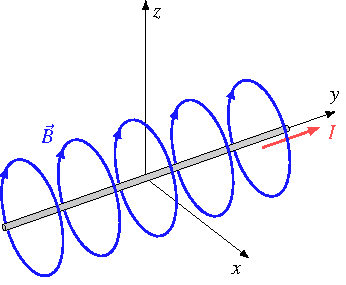
\includegraphics{papers/maxwell/images/mfeld.pdf}
% WIRE B FIELD 3D
	\caption{Magnetische Flussdichte um einen geraden Leiter}
	\label{maxwell:flussdichte}
\end{figure}




\subsubsection{Magnetisches Vektorpotential}

Wie in der Elektrostatik, gibt es auch in der Magnetostatik ein Potential, mit welchem energetische Zustände berechnet und ausgedrückt werden können. Im Unterschied ist jedoch das magnetische Potential ebenfalls eine vektorielle Grösse, also auch ein Vektorfeld. Das magnetische Vektorpotential zeigt jeweils in die selbe Richtung wie der Geschwindigkeitsvektor der bewegten Ladung.
Durch das magnetische Vektorpotential, kann die magnetische Flussdichte als 
\begin{equation}
	\operatorname{rot}\vec{A}=\nabla \times \vec{A}
	=
	\vec{B}
	\label{maxwell:definitionVektorpot}
\end{equation}
beschrieben werden, wobei wir dies für später bereits konkret ausrechnen wollen 
\begin{equation}
	\label{maxwell:nablaA}
	\renewcommand{\arraystretch}{1.9}
	\begin{pmatrix}
		\displaystyle
		\frac{\partial}{\partial x} \\
		\displaystyle
		\frac{\partial}{\partial y} \\
		\displaystyle
		\frac{\partial}{\partial z}
	\end{pmatrix}
	\times
	\begin{pmatrix}
		\displaystyle
		A_1 \\
		A_2 \\
		A_3 \\
	\end{pmatrix}
	=
	\begin{pmatrix}
		\displaystyle
		\frac{\partial A_3}{\partial y} -\frac{\partial A_2}{\partial z}\\
		\displaystyle
		\frac{\partial A_1}{\partial z} -\frac{\partial A_3}{\partial x}\\
		\displaystyle
		\frac{\partial A_2}{\partial x} -\frac{\partial A_1}{\partial y}
	\end{pmatrix}.
\end{equation}
Im Gegensatz zum elektrischen Feld, ist das magnetische Feld also kein Gradientenfeld seines Potentials, sondern ein Rotationsfeld.

Analog zur Elektrostatik, lässt sich mit dem magnetischen Vektorpotential die potentielle Energie der Wirkgrösse berechnen. Die Wirkgrösse ist jetzt allerdings keine ruhende Ladung $q$ mehr, sondern eine Ladung $q$ mit einer Geschwindigkeit $\vec{v}$, also eine bewegte Ladung. Explizit lässt sich die potentielle Energie als 
\[ W_{\text{p}} =  q\vec{v}\cdot\vec{A}\]
berechnen. Also das Skalarprodukt der Wirkgrösse und dem Potential des wirkenden Feldes an jenem Punkt im Raum.


%Mit dem Vektorpotential können ähnlich wie beim elektrischen Potential, energetische Zustände beschrieben werden. Die Wirkgrösse hier ist allerdings eine bewegte Ladung also eine Ladung $q$, welche eine Geschwindigkeit $\vec{v}$ hat. So kann das magnetische Potential dieser Grösse an einem Punkt berechnet werden. Zusätzlich ergibt sich über das Vektorpotential so auch die potentielle Energie dieser Wirkgrösse, auf welche weiter unten noch spezifischer eingegangen wird.


\subsection{Ampèresches Gesetz}
Das Ziel dieses Abschnitts ist erneut eine partielle Differentialgleichung zu finden, welche das Wesen des magnetischen Vektorpotentials und somit des magnetischen Feldes beschreibt.
Wiederum betrachten wir unter den oben vorausgesetzten Bedingungen einen luftleeren, dreidimensionalen Raum $V \subset \mathbb{R}^3$ in welchem das Vektorfeld des magnetischen Vektorpotentials $\vec{A}(x,y,z)$, somit das magnetische Feld $\vec{B}(x,y,z)$ und eine magnetische Wirkgrösse $q\vec{v}$  existieren. 

\subsubsection{Ansatz}

Wieder soll die Energie des gesamten Systems zusammengetragen und minimiert werden. 
Die Energiedichte des magnetischen Feldes mit \eqref{maxwell:definitionVektorpot} eingesetzt ist
\[ w_{\text{m}} 
= 
\frac{1}{2\mu_0}\vec{B}(x,y,z)^2
=
\frac{1}{2\mu_0}\left(\nabla\times\vec{A}(x,y,z)\right)^2. \]
Die Gesamtenergie jenes Feldes berechnet sich dann durch Integration über den gesamten Raum $V$ als
\begin{equation}
	\label{maxwell:magnetFeldEnergie}
	W_{\text{m}} = \iiint_V w_m\, dV\,.
\end{equation}
Wie bereits erwähnt, ergibt sich durch eine bewegte Ladung $q$ mit einer Geschwindigkeit $\vec{v}$ eine weitere potentielle Energie im System, welche sich als 
\[ 
W_{\text{p}}
= 
q\vec{v}
\cdot
\vec{A}
 \]
berechnen lässt.
Da unser Ziel jedoch ist, das Integral der Gesamtenergie zu minimieren, müssen wir auch diese potentielle Energie über den gesamten Raum bzw. das selbe Volumen integrieren wie das Integral in \eqref{maxwell:magnetFeldEnergie}. 

Dafür betrachten wir erneut nur ein kleines, ein infinitesimales Stück der Ladung also $dq\,\vec{v}$ und können mithilfe von $dq = \varrho\,dV$, wobei $\varrho$ die Ladungsdichte ist, dieses kleine Stück der Ladung sofort zu $\vec{v}\varrho\,dV$ umschreiben.
Wenn wir uns jetzt überlegen, dass sich eine Ladungsdichte mit einer Geschwindigkeit $\vec{v}$ bewegt, können wir auch sagen, dass dies äquivalent zu einer Stromdichte $\vec{\jmath}=\varrho\vec{v}$ ist. 
Die kleinen bzw. infinitesimalen Stücke der Wirkgrösse formen wir also zu \[\vec{\jmath}\,dV = \varrho\vec{v}\,dV\]
um und erhalten mit einer Integration über den ganzen Raum $V$
\begin{equation}
	W_{\text{p}}
	= 
	\iiint_V \vec{A}\cdot\varrho\vec{v}\,dV
	=
	\iiint_V \vec{A}(x,y,z)\cdot\vec{j}(x,y,z)\,dV
\end{equation}
die gesamte potentielle Energie der Wirkgrösse.

Jetzt befinden sich beide Energiekomponenten in einer Form, in welcher wir über denselben Raum bzw. dasselbe Volumen integrieren können und somit lassen sie sich zu einem einzigen Integral als 
\begin{align*}
W_{\text{tot}} 
&=
W_{\text{p}} - W_{\text{m}}
=
\iiint_V \vec{A}\cdot\vec{\jmath}
- \frac{1}{2\mu_0}\left(\nabla\times\vec{A}\right)\cdot\left(\nabla\times\vec{A}\right)\, dV \\
&=
\iiint_V \left( A_1j_1 + A_2j_2 + A_3j_3\right) - 
 \frac{1}{2\mu_0}\biggl( 
 	\biggl( \frac{\partial A_3}{\partial y} -\frac{\partial A_2}{\partial z}\biggr)^2 
 + \biggl( \frac{\partial A_1}{\partial z} -\frac{\partial A_3}{\partial x}\biggr)^2
 + \biggl(\frac{\partial A_2}{\partial x} -\frac{\partial A_1}{\partial y} \biggr)^2   
 \biggr) \,dV
\end{align*}
zusammenfassen.

In dieser Gleichung wird sofort das zu minimierende Integral ersichtlich und die Lagrange-Funktion kann als 

	%\begin{align}
	%\label{maxwell:magnetostatikLagrange}
	%L\left(x,y,z, \vec{A}, \vec{A}_x. \vec{A}_y, \vec{A}_z\right)
	%=&\left( A_1j_1 + A_2j_2 + A_3j_3\right) \\ \nonumber
	% &- \frac{1}{2\mu_0}\left( 
	%\left( \frac{\partial A_3}{\partial y} -\frac{\partial A_2}{\partial %z}\right)^2 
	%+ \left( \frac{\partial A_1}{\partial z} -\frac{\partial A_3}{\partial x}\right)^2
	%+ \left(\frac{\partial A_2}{\partial x} -\frac{\partial A_1}{\partial y} \right)^2   
	%\right)	
	%\end{align}
	
	\begin{align}
	\label{maxwell:magnetostatikLagrange}
	L\left(x,y,z, \vec{A}, \vec{A}_x. \vec{A}_y, \vec{A}_z\right)
	=&\left( A_1j_1 + A_2j_2 + A_3j_3\right) \\ \nonumber
	 &- \frac{1}{2\mu_0}\bigl( 
	( A_{3,y} - A_{2,z})^2 
	+ (A_{1,z} -A_{3,x})^2
	+ (A_{2,x} -A_{1,y})^2   
	\bigr)
	\end{align}
abgelesen und definiert werden. 
Hierbei wollen wir darauf hinweisen, dass die Lagrange-Funktion in diesem Fall von einem Vektor, dem magnetischen Vektorpotential $\vec{A}$ abhängig ist. 
Das bedeutet, dass jede Komponente des Vektorpotentials einzeln variiert werden kann, was später die Ursache für mehrere Ausführungen der Euler-Ostrogradski-Differentialgleichung sein wird.

Erneut stellen wir auch fest, dass ein additiver Term dazugekommen ist, wie weiter oben beschrieben handelt es sich auch um einen Kopplungsterm, welcher hier jedoch die Wechselwirkung zwischen dem Feld $\vec{A}$ und der Wirkgrösse, also der Stromdichte $\vec{\jmath}\,$ beschreibt.

\subsubsection{Einsetzen in die Euler-Ostrogradski-Differentialgleichung}

Da jede Komponente des magnetischen Vektorpotentials für sich variiert werden kann, resultieren demnach drei Euler-Ostrogradski-Differentialgleichungen der Form
\[ 
\frac{\partial L}{\partial A_i} 
- \frac{\partial}{\partial x}\frac{\partial L}{\partial A_{i,x}}
- \frac{\partial}{\partial y}\frac{\partial L}{\partial A_{i,y}}
- \frac{\partial}{\partial z}\frac{\partial L}{\partial A_{i,z}}
= 0 \qquad \text{für } i=1,2,3
\, . \]
{\larger\textcircled{\smaller[2]1}} $i = 1$:
\begin{subequations}
	\label{maxwell:magnetoL1}
\begin{gather}
	0
	=
	j_1 - \underbrace{\frac{\partial}{\partial x}\frac{\partial L}{\partial A_{1,x}}}_{=0}
	 - \left( \frac{1}{2\mu_0}(-1)\,2 \frac{\partial}{\partial y}(A_{2,x}-A_{1,y})\right) 
	 - \left( \frac{1}{2\mu_0}\,2\frac{\partial}{\partial z}(A_{1,z}-A_{3,x})\right)
	 \\
	 0
	 =
	 j_1 - \frac{1}{\mu_0}\left( \frac{\partial}{\partial y}(A_{2,x}-A_{1,y})
	 - \frac{\partial}{\partial z}(A_{1,z}-A_{3,x})
	 \right)  
	 \\	 
	 \mu_0j_1
	 =
	 \frac{\partial}{\partial y}(A_{2,x}-A_{1,y})
	 - \frac{\partial}{\partial z}(A_{1,z}-A_{3,x})	 	 	 
\end{gather}
\end{subequations}
{\larger\textcircled{\smaller[2]2}} $i = 2$:
\begin{equation}
	\label{maxwell:magnetoL2}
	\mu_0j_2
	=
	\frac{\partial}{\partial z}(A_{3,y}-A_{2,z})
	- \frac{\partial}{\partial x}(A_{2,x}-A_{1,y})
\end{equation}
{\larger\textcircled{\smaller[2]3}} $i = 3$:
\begin{equation}
	\label{maxwell:magnetoL3}
	\mu_0j_3
	=
	\frac{\partial}{\partial x}(A_{1,z}-A_{3,x})
	- \frac{\partial}{\partial y}(A_{3,y}-A_{2,z})
\end{equation}
Wobei für $i=2,3$ genau das gleiche Vorgehen wie bei $i=1$ angewendet wurde.
Mithilfe von \eqref{maxwell:nablaA} wollen wir jetzt den Ausdruck $\nabla\times\nabla\times\vec{A} = \nabla\times\vec{B}$ betrachten.

\begin{equation}
	\renewcommand{\arraystretch}{1.9}
	\begin{pmatrix}
		\displaystyle
		\frac{\partial}{\partial x} \\
		\displaystyle
		\frac{\partial}{\partial y} \\
		\displaystyle
		\frac{\partial}{\partial z}
	\end{pmatrix}
	\times
	\begin{pmatrix}
		\displaystyle
		\frac{\partial A_3}{\partial y} -\frac{\partial A_2}{\partial z}\\
		\displaystyle
		\frac{\partial A_1}{\partial z} -\frac{\partial A_3}{\partial x}\\
		\displaystyle
		\frac{\partial A_2}{\partial x} -\frac{\partial A_1}{\partial y}
	\end{pmatrix}
	=
	\begin{pmatrix}
		\displaystyle
		\frac{\partial}{\partial y}(A_{2,x}-A_{1,y}) - \frac{\partial}{\partial z}(A_{1,z}-A_{3,x})	\\
		\displaystyle
		\frac{\partial}{\partial z}(A_{3,y}-A_{2,z}) - \frac{\partial}{\partial x}(A_{2,x}-A_{1,y}) \\
		\displaystyle
		\frac{\partial}{\partial x}(A_{1,z}-A_{3,x}) - \frac{\partial}{\partial y}(A_{3,y}-A_{2,z})
	\end{pmatrix}
\end{equation}
Wir stellen fest, dass die drei Komponenten des resultierenden Vektors genau mit den rechten Seiten der drei Gleichungen \eqref{maxwell:magnetoL1}, \eqref{maxwell:magnetoL2} und \eqref{maxwell:magnetoL3} übereinstimmen.
Dank der kompakten vektoriellen Schreibweise, können wir also unser Ergebnis der genannten drei Gleichungen zu
\[ 
\mu_0\vec{\jmath} 
= 
\nabla \times \vec{B}
 \]
zusammenfassen. Hierbei resultiert das ampèresche Gesetz.

\subsubsection{Interpretation des Resultates}

Mittels der Variationsrechnung konnten wir das ampèresche Gesetz herleiten, welches besagt, dass die Stromdichte proportional zur Rotation des magnetischen Feldes ist. Anders ausgedrückt kann man auch sagen, dass die Stromdichte, welche durch eine Fläche strömt, proportional zum magnetischen Feld ist, welches um den Rand dieser selben Fläche wirkt.



%
% einleitung.tex -- Beispiel-File für die Einleitung
%
% (c) 2020 Prof Dr Andreas Müller, Hochschule Rapperswil
%
% !TEX root = ../../buch.tex
% !TEX encoding = UTF-8
%
%Elektrodynmaik

\section{Elektrodynamik\label{section:maxwell:elektrodynmaik}}
\rhead{Elektrodynamik}
In der Elektrodynamik erlauben wir, dass
\[
\frac{\partial f}{\partial t}
\neq
0
\]
für die Funktionen, die wir betrachten, gelten darf.
Das heisst Ladungen dürfen sich nun mit einer beliebigen Geschwindigkeit $\vec{v}$ bewegen und wir berücksichtigen zeitabhängige Skalar- und Vektorfelder.
Bei den statischen Maxwell-Gleichungen fällt auf, dass das elektrische und magnetische Feld keinerlei Abhängigkeiten voneinander haben.
Wie sich später herausstellen wird, ändert sich dies, denn die Zeitabhängigkeit führt dazu, dass sich das elektrische und magnetische Feld gegenseitig beeinflussen.
Daraus folgen einige spannende Tatsachen, auf die wir später noch zu sprechen kommen.
 
Im folgenden werden wir unseren Raum definieren und bekannte Vektorfelder in ihrer Definition anpassen.

\subsubsection{Der vierdimensionale Raum}
Der Raum in dem wir uns nun bewegen, definieren wir als
\begin{equation}
	\Omega
	=
	\begin{pmatrix}
		ct\\
		x\\
		y\\
		z
	\end{pmatrix}
	=
	\Omega^{\mu} \subset \mathbb{R}^4,
\end{equation}
wobei $\Omega^0$ die Zeit $t$ multipliziert mit der Lichtgeschwindigkeit
\[
c
=
\frac{1}{\sqrt{\varepsilon_0\,\mu_0\mathstrut}}
\]
ist.
Damit wir uns später ein wenig Schreibaufwand sparen können, schreiben wir die Ableitungen der Raumkomponenten als
\[
\frac{\partial}{\partial \Omega^{\mu}}
=
\partial^{\mu}.
\]

\subsubsection{4er Gradient}
Der 4er Gradient einer Funktion $f: \mathbb{R}^4 \rightarrow \mathbb{R}$ im Raum $\Omega$ ist von der Form
\[
\renewcommand{\arraystretch}{1.9}
\nabla^\mu f
=
\begin{pmatrix}
	\displaystyle
	\partial^0 f\\
	\displaystyle
	\partial^1 f\\
	\displaystyle
	\partial^2 f\\
	\displaystyle
	\partial^3 f
\end{pmatrix}
=
\begin{pmatrix}
	\displaystyle
	\frac{\partial f}{\partial (ct)}\\
	\displaystyle
	\frac{\partial f}{\partial x}\\
	\displaystyle
	\frac{\partial f}{\partial y}\\
	\displaystyle
	\frac{\partial f}{\partial z}
\end{pmatrix}
=
\begin{pmatrix}
	\displaystyle
	\frac{1}{c}\frac{\partial f}{\partial t}\\
	\displaystyle
	\frac{\partial f}{\partial x}\\
	\displaystyle
	\frac{\partial f}{\partial y}\\
	\displaystyle
	\frac{\partial f}{\partial z}
\end{pmatrix}
=
\begin{pmatrix}
	\displaystyle
	\frac{1}{c}\frac{\partial f}{\partial t}\\
	\displaystyle
	\nabla f
\end{pmatrix}.
\]


\subsubsection{Dynamisches elektrisches Feld}
Das elektrische Feld
\(
\vec{E}: \mathbb{R}^4 \rightarrow \mathbb{R}^3
\)
wird in der Elektrodynamik definiert als
\begin{equation}
	\vec{E}(t,x,y,z)
	=
	- \nabla\varphi(t,x,y,z) - \frac{\partial \vec{A}}{\partial t}(t,x,y,z).
	\label{maxwell:section:definiton_dynamisch_elektrischesFeld}
\end{equation}
Es fällt auf, dass das elektrische Feld, das elektrische Potentialfeld und das magnetische Vektorpotential nun einen vierdimensionalen Inputvektor besitzen, wobei die zusätzliche Dimension die Zeit ist. 

\subsubsection{Dynamisches magnetisches Feld}
Das magnetische Feld
\(
\vec{B}: \mathbb{R}^4 \rightarrow \mathbb{R}^3
\)
wird in der Elektrodynamik ähnlich definiert wie in der Magnetostatik. Nämlich als
\begin{equation}
	\vec{B}(t,x,y,z)
	=
	\nabla \times \vec{A}(t,x,y,z).
	\label{maxwell:section:definition_dynamisch_magnetischesFeld}
\end{equation}
Der Unterschied liegt hier einzig in der zusätzlichen Zeitkomponente im Inputvektor.

\subsection{Dynamische Maxwell-Gleichungen}
Das Ziel dieses Abschnitts ist ein Variationsprinzip zu formulieren, welches uns die Verhaltensgleichungen der Elektrodynamik liefert. 
Wir betrachten nun den luftleeren, vierdimensionalen Raum $\Omega$.
In diesem Raum existieren nun das elektrische Feld $\vec{E}(t,x,y,z)$, das magnetische Feld $\vec{B}(t,x,y,z)$, eine Stromdichte $\vec{\jmath}(t,x,y,z)$ und eine zeitunabhängige Ladungsdichte $\varrho(x,y,z)$.

\subsubsection{Ansatz}
Wir wählen einen ähnlichen Ansatz wie bislang, nämlich ein Integral über die Zeit der Energie im Raum zu minimieren.
Das Integral über die Zeit ist notwendig, da wir über alle Inputgrössen integrieren müssen.
Diese neue Grösse werden wir mit $D$ bezeichnen.
Durch Superponierung unserer bisher gefundenen Energien erhalten wir
\begin{align*}
	D
	&=
	\int_{(ct)_0}^{(ct)_1} W_{\text{tot}}\,d(ct)
	=
	\int_{t_0}^{t_1} \left(W_{\text{e}} - W_{\text{q}} + W_{\text{p}} - W_{\text{m}}\right)c\,dt
	\\
	&= \int_{\Omega} \frac{1}{2}\,\varepsilon_0\,\vec{E}\,^2 - \varphi\,\varrho 
	+ \vec{A}\cdot\vec{\jmath} - \frac{1}{2\mu_0}\vec{B}^2 \,d\Omega.
\end{align*}
Man sieht hier sehr schön, wie die Feldenergie aus dem Term
\[
w_{\text{e}} - w_{\text{m}}
=
\frac{1}{2}\,\varepsilon_0\,\vec{E}^2 - \frac{1}{2\,\mu_0}\vec{B}^2
\]
besteht und die Kopplungsterme 
\(
\varphi\,\varrho
\)
und
\(
\vec{A}\cdot\vec{\jmath}
\)
sind.
Hiermit ist es uns allerdings noch nicht gelungen ein Energiefunktional zu formulieren, welches von der Form
\[
I(f) = \int_{t_0}^{t_1} \int_{z_0}^{z_1} \int_{y_0}^{y_1} \int_{x_0}^{x_1} L(t,x,y,z,f,f_t,f_x,f_y,f_z)\,dx\,dy\,dz\,dt 
\]
ist, weil das elektrische und magnetische Feld von unterschiedlichen Potentialen abhängig sind.

\subsubsection{Elektromagnetisches 4er Potential}
An dieser Stelle führen wir ein neues Vektorfeld ein, welches die Potentiale des elektrischen und magnetischen Feldes beinhaltet.
Dieses neue Vektorfeld heisst elektromagnetisches 4er Potential
\(
A:\mathbb{R}^4 \rightarrow \mathbb{R}^4
\)
und wird als
\begin{equation}
	A
	=
	\begin{pmatrix}
		\varphi / c\\
		A_x\\
		A_y\\
		A_z
	\end{pmatrix}
	=
	A^{\mu},
\end{equation}
definiert, wobei $A_x$, $A_y$, $A_z$ die Komponenten des magnetischen Vektorpotentiales $\vec{A}$ sind.
Mittels dieser Grösse können wir nun das elektrische und magnetische Feld ausdrücken.
Also
\begin{equation}
\frac{1}{c}\, \vec{E}
=
-\frac{1}{c}\, \nabla\,\varphi - \frac{1}{c}\,\frac{\partial \vec{A}}{\partial t}
=
\begin{pmatrix}
	-\partial^1 A^0 - \partial^0 A^1\\
	-\partial^2 A^0 - \partial^0 A^2\\
	-\partial^3 A^0 - \partial^0 A^3
\end{pmatrix}
=
\begin{pmatrix}
	E_x / c\\
	E_y / c\\
	E_z / c
\end{pmatrix}
\end{equation}
und
\begin{equation}
\vec{B}
=
\nabla \times \vec{A}
=
\begin{pmatrix}
	\partial^2 A^3 - \partial^3 A^2\\
	\partial^3 A^1 - \partial^1 A^3\\
	\partial^1 A^2 - \partial^2 A^1
\end{pmatrix}
=
\begin{pmatrix}
	B_x\\
	B_y\\
	B_z
\end{pmatrix}.
\end{equation}
Daraus ergibt sich für die Feldenergiedichten
\[
w_{\text{e}}
=
\frac{1}{2}\underbrace{\varepsilon_0\,c^2}_{\displaystyle=1/\mu_0} \biggl(\left(\partial^0 A^1 + \partial^1 A^0\right)^2 + \left(\partial^0 A^2 + \partial^2 A^0\right)^2 + 
\left(\partial^0 A^3 + \partial^3 A^0\right)^2\biggr)
\]
und 
\[
w_{\text{m}}
=
\frac{1}{2\mu_0}\,\biggl(\left(\partial^2 A^3 - \partial^3 A^2\right)^2 + \left(\partial^3 A^1 - \partial^1 A^3\right)^2 + 
\left(\partial^1 A^2 - \partial^2 A^1\right)^2\biggr).
\]

\subsubsection{4er Stromdichte}
Damit wir nun auch die Kopplungsterme mit dem elektromagnetischen 4er Potential ausdrücken können, führen wir die 4er Stromdichte
\(
J:\mathbb{R}^4 \rightarrow \mathbb{R}^4
\)
ein. Wir definieren sie als
\begin{equation}
J
=
\begin{pmatrix}
	-c\varrho\\
	j_x\\
	j_y\\
	j_z
\end{pmatrix}
=
J^{\mu},
\end{equation}
wobei $j_x$, $j_y$ und $j_z$ die Komponenten der Stromdichte $\vec{\jmath}$ sind.
Somit können wir unsere beiden Kopplungsterme schön kompakt  als
\begin{equation}
	w_{\text{p}} - w_{\text{q}}
	=
	J\cdot A
\end{equation}
schreiben.

\subsubsection{Formulierung der Lagrange-Funktion}
Uns ist es nun gelungen die Grösse $D$ mit einer Funktion und ihren partiellen Ableitungen zu formulieren.
Es ist nämlich 
\begin{align*}
D
=
\int_{\Omega}
\frac{1}{2\mu_0}\,\biggl(\left(\partial^0 A^1 + \partial^1 A^0\right)^2 + \left(\partial^0 A^2 + \partial^2 A^0\right)^2 + 
\left(\partial^0 A^3 + \partial^3 A^0\right)^2\biggr) \\
-  \frac{1}{2\mu_0}\,\biggl(\left(\partial^2 A^3 - \partial^3 A^2\right)^2 + \left(\partial^3 A^1 - \partial^1 A^3\right)^2 + 
\left(\partial^1 A^2 - \partial^2 A^1\right)^2\biggr)\\
+ J^0 A^0 + J^1 A^1 + J^2 A^2 + J^3 A^3 \,d\Omega
\end{align*}
und somit die Lagrange-Funktion
\begin{align*}
L(\Omega^0,...,\Omega^3, A^0,...,A^3, \partial^0 A^i,...,\partial^3 A^i)
=
\frac{1}{2\mu_0}\,\biggl(\left(\partial^0 A^1 + \partial^1 A^0\right)^2 + \left(\partial^0 A^2 + \partial^2 A^0\right)^2 + 
\left(\partial^0 A^3 + \partial^3 A^0\right)^2\biggr) \\
-  \frac{1}{2\mu_0}\,\biggl(\left(\partial^2 A^3 - \partial^3 A^2\right)^2 + \left(\partial^3 A^1 - \partial^1 A^3\right)^2 + 
\left(\partial^1 A^2 - \partial^2 A^1\right)^2\biggr)\\
+ J^0 A^0 + J^1 A^1 + J^2 A^2 + J^3 A^3.
\end{align*}

\subsubsection{Einsetzen in die Euler-Ostrogradski-Differentialgleichung}
Da unsere Lagrange-Funktion wiederum von einer vektoriellen Grösse abhängig ist, erhalten wir diesmal vier Euler-Ostrogradski-Differentialgleichungen von der Form
\[
\frac{\partial L}{\partial A^i} 
- \frac{\partial}{\partial \Omega^0}\frac{\partial L}{\partial(\partial^0 A^i)}
- \frac{\partial}{\partial \Omega^1}\frac{\partial L}{\partial(\partial^1 A^i)}
- \frac{\partial}{\partial \Omega^2}\frac{\partial L}{\partial(\partial^2 A^i)}
- \frac{\partial}{\partial \Omega^3}\frac{\partial L}{\partial(\partial^3 A^i)}
= 0 \qquad \text{für } i=0,1,2,3.
\]
{\larger\textcircled{\smaller[2]1}} $i = 0$:
\[
J^0  -\frac{1}{\mu_0}\,\biggl(\partial^1\underbrace{\left(\partial^0 A^1 + \partial^1 A^0\right)}_{\displaystyle=-E_x/c}
+ \partial^2\underbrace{\left(\partial^0 A^2 + \partial^2 A^0\right)}_{\displaystyle=-E_y/c}
+ \partial^3\underbrace{\left(\partial^0 A^3 + \partial^3 A^0\right)}_{\displaystyle=-E_z/c}\biggr)
=
0
\]
{\larger\textcircled{\smaller[2]2}} $i = 1$:
\[
J^1  -\frac{1}{\mu_0}\,\biggl(\partial^0\underbrace{\left(\partial^0 A^1 + \partial^1 A^0\right)}_{\displaystyle=-E_x/c}
+ \underbrace{\partial^2\left(\partial^1 A^2 + \partial^2 A^1\right)
	- \partial^3\left(\partial^3 A^1 + \partial^1 A^3\right)}_{\displaystyle=(\nabla\times\vec{B})_x}\biggr)
=
0
\]
{\larger\textcircled{\smaller[2]3}} $i = 2$:
\[
J^2  -\frac{1}{\mu_0}\,\biggl(\partial^0\underbrace{\left(\partial^0 A^2 + \partial^2 A^0\right)}_{\displaystyle=-E_y/c}
+ \underbrace{\partial^3\left(\partial^2 A^3 + \partial^3 A^2\right)
	- \partial^1\left(\partial^1 A^2 + \partial^2 A^1\right)}_{\displaystyle=(\nabla\times\vec{B})_y}\biggr)
=
0
\]
{\larger\textcircled{\smaller[2]4}} $i = 3$:
\[
J^3  -\frac{1}{\mu_0}\,\biggl(\partial^0\underbrace{\left(\partial^0 A^3 + \partial^3 A^0\right)}_{\displaystyle=-E_z/c}
+ \underbrace{\partial^1\left(\partial^3 A^1 + \partial^1 A^3\right)
	- \partial^2\left(\partial^2 A^3 + \partial^3 A^2\right)}_{\displaystyle=(\nabla\times\vec{B})_z}\biggr)
=
0
\]
Für $i=0$ resultiert die partielle Differentialgleichung
\begin{align}
-c\varrho + \frac{1}{\mu_0\,c}\,\biggl(\frac{\partial E_x}{\partial x}
+ \frac{\partial E_y}{\partial y} + \frac{\partial E_z}{\partial z}\biggr)
&=
0\\[1em]
\Leftrightarrow \qquad \nabla\cdot\vec{E}
&=
\frac{\varrho}{\varepsilon_0},
\label{maxwell:section:gauss_dynamisch}
\end{align}
was dem dynamischen gaussschen Gesetz des elektrischen Feldes entspricht.
Für $i=1,2,3$ resultiert das partielle Differentialgleichungssystem
\begin{align}
\vec{\jmath} + \frac{1}{\mu_0\,c^2}\frac{\partial \vec{E}}{\partial t}
- \frac{1}{\mu_0}\nabla\times\vec{B}
&=
0\\[1em]
\Leftrightarrow \qquad \varepsilon_0\,\mu_0\frac{\partial \vec{E}}{\partial t} + \mu_0\vec{\jmath}
&=
\nabla\times\vec{B},
\label{maxwell:section:ampere_dynamisch}
\end{align}
was dem dynamischen ampèreschen Gesetz entspricht.
 
Wir kommen nun zur Erkenntnis, dass man die fundamentalen Feldgleichungen des Elektromagnetismus mit einem Variationsprinzip herleiten kann.
Dafür mussten wir nur die Feldenergien und Wechselwirkungen mit einem Funktional ausdrücken und dieses mithilfe der Variationsrechnung minimieren.
Eine wunderschöne Tatsache, denn einmal mehr wurden wir Zeuge davon, dass wenn wir Energien minimieren, Naturgesetze resultieren!

\subsubsection{Interpretation der Resultate}
Was können wir aus diesen zwei partiellen Differentialgleichungen entnehmen?
In der Gleichung \eqref{maxwell:section:gauss_dynamisch} sehen wir, dass das gausssche Gesetz im statischen wie auch im dynamischen Fall von der gleichen Form ist.
Das heisst die Quelle des elektrischen Feldes ist eine Ladungsdichte $\varrho$.
In der Gleichung \eqref{maxwell:section:ampere_dynamisch} fällt auf, dass das dynamische ampèrsche Gesetz, im Vergleich zum statischen, einen zusätzlichen Term erhalten hat, der eine zeitliche Veränderung des elektrischen Feldes beschreibt.
Also verursacht nicht nur eine Stromdichte, sondern auch eine zeitliche Veränderung im elektrischen Feld eine Rotation im magnetischen Feld.
An dieser Stelle bemerken wir zum ersten Mal, dass das magnetische Feld vom elektrischen Feld beeinflusst werden kann.


\subsubsection{Gausssches Gesetz des magnetischen Feldes und faradaysches Gesetz der Induktion}
Der Vollständigkeit halber wollen wir noch einige Worte über die bisher nicht explizit erwähnten Maxwell-Gleichungen verlieren.
Die beiden Gesetze folgen ganz trivial aus der Definition des elektrischen und magnetischen Feldes.
 
Wenn wir in der Gleichung \eqref{maxwell:section:definition_dynamisch_magnetischesFeld} auf beiden Seiten die Divergenz anwenden, erhalten wir
\[
\nabla \cdot \vec{B}
=
\nabla \cdot (\nabla \times \vec{A}).
\]
Da die Divergenz eines Rotationsfeldes immer null ist, folgt direkt, dass
\begin{equation}
\nabla \cdot \vec{B}
=
0
\label{maxwell:section:Gauss_magnetisches_Feld}
\end{equation}
gelten muss.
Dies entspricht dem gaussschen Gesetz des magnetischen Feldes.
Es besagt, dass das magnetische Feld quellenfrei ist oder anders ausgedrückt, dass keine magnetische Monopole existieren. Was wiederum auch bedeutet, dass die magnetischen Feldlinien immer in sich geschlossen sein müssen.
 
Wenn wir in der Gleichung \eqref{maxwell:section:definiton_dynamisch_elektrischesFeld} auf beiden Seiten die Rotation anwenden, erhalten wir
\[
\nabla \times \vec{E}
=
\nabla \times \left(- \nabla \varphi\right) - \nabla \times \biggl(\frac{\partial \vec{A}}{\partial t}\biggr).
\]
Wir sehen direkt, dass die Rotation eines Gradientenfeldes immer null ist und somit verschwindet der erste Term.
Da die partielle Ableitung nach der Zeit eine lineare Operation ist, können wir die Reihenfolge der Operationen im zweiten Term vertauschen und die Gleichung wird zu
\begin{equation}
\nabla \times \vec{E}
=
- \frac{\partial}{\partial t} (\nabla \times \vec{A})
=
- \frac{\partial \vec{B}}{\partial t}.
\end{equation}
Was wir erhalten ist das faradaysche Gesetz der Induktion.
Diese partiellen Differentialgleichungen sagen uns, dass eine zeitliche Veränderung des magnetischen Feldes eine Rotation des elektrischen Feldes verursacht. Also sehen wir, dass auch das elektrische Feld vom magnetischen Feld beeinflusst werden kann. Da in der Elektrodynamik eine zeitliche Veränderung in einem Feld eine Rotation im anderen Feld zur Folge hat, ist die Existenz von elektromagnetischen Wellen so auch intuitiv naheliegend. 


\subsubsection{Exkurs zu elektromagnetischen Wellen}

\begin{figure}
	\centering
	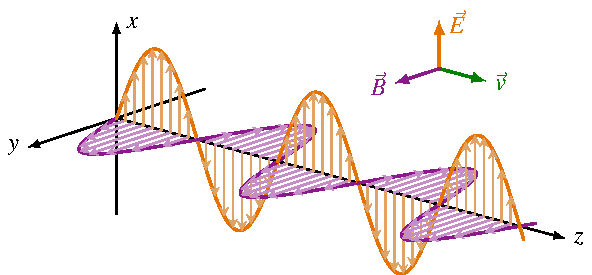
\includegraphics{papers/maxwell/images/emwelle.pdf}
	\caption{Elektromagnetische Welle im Vakuum}
	\label{maxwell:section:bild_em_welle}
\end{figure}
In einem luftleeren Raum, in welchem keine Stromdichte $\vec{\jmath}$ und keine Ladungsdichte $\varrho$ existieren, gilt
\begin{align}
\nabla \times \vec{B}
&=
\varepsilon_0\,\mu_0 \frac{\partial \vec{E}}{\partial t}
\label{maxwell:section:ampere_vakuum}
\\
\nabla \times \vec{E}
&=
-\frac{\partial \vec{B}}{\partial t}.
\label{maxwell:section:faraday_vakuum}
\end{align}
Nun können wir in Gleichung \eqref{maxwell:section:ampere_vakuum} die Rotation auf beiden Seiten anwenden und mithilfe der Grassmann-Identität resultiert
\begin{align*}
\nabla \times \nabla \times \vec{B}
&=
\varepsilon_0\,\mu_0 \frac{\partial}{\partial t} (\nabla \times \vec{E})\\
\Leftrightarrow \qquad \nabla \underbrace{(\nabla \cdot \vec{B})}_{\displaystyle=0} - \Delta \vec{B}
&=
-\varepsilon_0\,\mu_0 \frac{\partial ^2 \vec{B}}{\partial t^2}\\
\Leftrightarrow \qquad \frac{\partial ^2 \vec{B}}{\partial t^2}
&=
\underbrace{\frac{1}{\varepsilon_0\,\mu_0}}_{\displaystyle=c^2} \Delta \vec{B}.
\end{align*}
Dies entspricht genau der Wellengleichung.
Mit dem gleichen Vorgehen resultiert für die Gleichung \eqref{maxwell:section:faraday_vakuum}
\begin{align*}
\nabla \times \nabla \times \vec{E}
&=
- \frac{\partial}{\partial t} (\nabla \times \vec{B})\\
\Leftrightarrow \qquad \nabla \underbrace{(\nabla \cdot \vec{E})}_{\displaystyle=0} - \Delta \vec{E}
&=
- \varepsilon_0\,\mu_0 \frac{\partial ^2 \vec{E}}{\partial t^2}\\
\Leftrightarrow \qquad \frac{\partial ^2 \vec{E}}{\partial t^2}
&=
\underbrace{\frac{1}{\varepsilon_0\,\mu_0}}_{\displaystyle=c^2} \Delta \vec{E}.
\end{align*}
Wir kommen also zum Schluss, dass beide Felder die Wellengleichung im genannten Raum erfüllen. Eine Lösung der Wellengleichung kann wie in Abbildung \ref{maxwell:section:bild_em_welle} aussehen. Was dabei auffällt ist, dass die Ausbreitungsgeschwindigkeit in beiden Fällen die Lichtgeschwindigkeit $c$ ist. 
%Daraus kann man schliessen, dass Licht eine elektromagnetische Welle ist.
Daraus kann man erahnen und plausibilisieren, dass Licht eine elektromagnetische Welle ist. 



\input{papers/maxwell/schluss.tex}


\printbibliography[heading=subbibliography]

\end{refsection}
